\documentclass[a4paper, 11pt]{article}
\usepackage{comment}
\usepackage{fullpage}
\usepackage{amsmath}
\usepackage{amssymb}
\usepackage{mathtools}
\usepackage{fontspec}
\defaultfontfeatures{Ligatures=TeX}
\usepackage{xfrac}
\usepackage{icomma}
\usepackage[section,below]{placeins}
\usepackage[labelfont=bf,font=small,width=0.9\textwidth]{caption}
\usepackage{subcaption}
\usepackage{graphicx}
\usepackage{grffile}
\usepackage{float}
\floatplacement{figure}{htbp}
\floatplacement{table}{htbp}
\usepackage{booktabs}
\usepackage{hyperref}
\usepackage[ngerman]{babel}
\usepackage[final]{pdfpages}

\DeclarePairedDelimiter{\ev}{\langle}{\rangle}
\begin{document}
\noindent
%\centerline{\small{\textsc{Technische Universität Dortmund}}} \\
\large{\textbf{2. Übungsblatt zur Vorlesung \hfill WS 2017/2018 \\
Statistische Methoden der Datenanalyse \hfill Prof. W. Rhode}} \\
Annika Burkowitz, Sebastian Bange, Alexander Harnisch \\
\noindent\makebox[\linewidth]{\rule{\textwidth}{0.4pt}}

\section*{Aufgabe 5}
In dieser Aufgabe wird die \textsc{Maxwell}'sche Geschwindigkeitsverteilung in der Form
\begin{equation}
    f(v) = N 4 \pi v^2 \exp\left(-\frac{mv^2}{2k_\textup{B}T}\right)
    \label{eqn:f}
\end{equation}
betrachtet. Zuerst ist die Verteilung zu normieren. Dafür kann die Gammafunktion verwendet werden, es geht aber auch viel schöner ohne. Dafür definieren wir zuerst
\begin{equation}
    I := \int_{0}^{\infty} \exp(-\alpha t x^2)\textup{d}x\,.
    \label{eqn:I}
\end{equation}
Um $I$ auszuwerten wird quadriert und anschließend in Polarkoordinaten gewechselt:
\begin{align}
    I^2 &= \left(\int_{0}^{\infty} \exp(-\alpha tx^2)\textup{d}x\right)\left(\int_{0}^{\infty} \exp(-\alpha tx^2)\textup{d}x\right) \\
    &= \int_{0}^{\infty}\int_{0}^{\infty} \exp(-\alpha t(x^2 + y^2))\textup{d}x \textup{d}y \\
    &= \int_{0}^{\pi/2}\textup{d}\phi\int_{0}^{\infty}\exp(-\alpha t r^2)r \textup{d}r \\
    &= \frac{\pi}{4} \int_{0}^{\infty} \exp(-\alpha t u) \textup{d} u \\
    &= \frac{\pi}{4\alpha t} \,.
\end{align}
Wegen $I > 0$ ergibt sich somit
\begin{equation}
    I = \sqrt{I^2} = \frac{1}{2} \sqrt{\frac{\pi}{\alpha t}}\,.
    \label{eqn:I_sol}
\end{equation}
Das für die Normierung zu berechnende Integral lässt sich nun auswerten:
\begin{equation}
    \int_{0}^{\infty} x^2\exp(-\alpha x^2) = - \frac{1}{\alpha} \frac{\textup{d}}{\textup{d}t} I\Big|_{t = 1} = \frac{1}{4}\sqrt{\pi}(\alpha t)^{-\frac{3}{2}}\Big|_{t=1} = \frac{\sqrt{\pi}}{4 \alpha^{\frac{3}{2}}} \,.
\end{equation}
Damit erhalten wir
\begin{align}
    \int_{0}^{\infty} f(v) \textup{d}v &= N 4 \pi \frac{\sqrt{\pi}}{4}\left(\frac{2k_{\textup{B}}T}{m}\right)^{\frac{3}{2}} \stackrel{\textup{!}}{=} 1 \\
    \Rightarrow N &= \left(\frac{m}{2\pi k_\textup{B}T}\right)^{\frac{3}{2}} \,.
    \label{eqn:N}
\end{align}

\subsection*{a)}
Die wahrscheinlichste Geschwindigkeit $v_\textup{m}$ ist die Stelle, an der $f$ maximal wird. Daher bilden wir die Ableitung
\begin{equation}
    \frac{\textup{d}}{\textup{d}v}f = 4\pi Nv\exp\left(-\frac{m v^2}{2 k_\textup{B}T}\right)\left(2 - \frac{mv^2}{k_\textup{B}T}\right) \stackrel{\textup{!}}{=} 0 \,.
\end{equation}
Das Extremum bei 0 ist offenbar ein Tiefpunkt, da $f$ keine negativen Werte annimmt und $f(0) = 0$. Daraus folgt, dass die beiden anderen Extrema Maxima sind, wobei das positive der beiden an der gesuchten Stelle
\begin{equation}
    v_\textup{m} = \sqrt{\frac{2 k_\textup{B} T}{m}}
    \label{eqn:v_m}
\end{equation}
liegt.

\subsection*{b)}
\label{subsec:b}
Der Erwartungswert des Geschwindigkeitsbetrags lässt sich wie folgt berechnen:
\begin{align}
    \ev{v}_f &= \int_{0}^{\infty} v f(v) \textup{d}v = 4\pi N \int_{0}^{\infty} v^3 \exp\left(-\frac{mv^2}{2k_\textup{B}T}\right) \textup{d}v \\
    &= 4\pi N \int_{0}^{\infty} \frac{u}{2} \exp\left(-\frac{mu}{2k_\textup{B}T}\right) \textup{d}u \\
    &= 2\pi N\left(\left[-\frac{2uk_\textup{B}T}{m}\exp\left(-\frac{mu}{2k_\textup{B}T}\right)\right]_{u=0}^{u=\infty} + \frac{2k_\textup{B}T}{m}\int_{0}^{\infty}\exp\left(-\frac{mu}{2k_\textup{B}T}\right) \textup{d}u\right) \\
    &= 2\pi N\left(\frac{k_\textup{B}T}{m}\right)^2 \stackrel{\eqref{eqn:N}}{=} 2 \sqrt{\frac{2k_\textup{B}T}{\pi m}} = \frac{2}{\sqrt{\pi}}v_\textup{m} \,.
\end{align}

\subsection*{c)}
Gesucht ist der Median $v_{0,5}$, für den gilt
\begin{equation}
    \int_{0}^{v_{0,5}} f(v) \textup{d}v = \frac{1}{2} \,.
    \label{eqn:median_int}
\end{equation}
Es ist nicht möglich, eine analytische Lösung für $v_{0,5}$ zu finden, da für $f(v)$ keine Stammfunktion gefunden werden kann. Daher lösen wir die Gleichung numerisch, dafür muss diese zuerst in eine dimensionslose Form gebracht werden. Mit dem vorherigen Ergebnis \eqref{eqn:v_m} gilt
\begin{equation}
    N = \pi^{-\frac{3}{2}}v_\textup{m}^{-3} \Rightarrow f(v) = \frac{4}{\sqrt{\pi}v_\textup{m}}\frac{v^2}{v_\textup{m}^2} \exp\left(-\frac{v^2}{v_\textup{m}^2}\right)\,.
\end{equation}
Mit der Substitution $x = \frac{v}{v_\textup{m}}$ nimmt \eqref{eqn:median_int} die für numerische Integration geeignete Form
\begin{equation}
    \int_{0}^{v_{0,5}} f(v) \textup{d}v = \frac{4}{\sqrt{\pi}} \int_{0}^{\frac{v_{0,5}}{v_\textup{m}}} x^2 e^{-x^2} \textup{d}x \stackrel{\textup{!}}{=} \frac{1}{2}
\end{equation}
an. Das Integral kann nun sukzessive mit einer beliebigen \textsc{Newton}-\textsc{Cotes}-Formel berechnet werden, bis es den gewünschten Wert von $\frac{1}{2}$ überschreitet. Wir verwenden die Trapezregel. Um den Performance-Limitierungen des \textsc{Python}-Interpreters möglichst gut zu entgehen, verwenden wir außerdem die Pakete \textsc{Numpy} bzw. \textsc{numexpr}. Es werden in einer Schleife immer $N$ Funktionsauswertungen parallelisiert durchgeführt und die Teilsummen anschließend aufsummiert. Für optimale Performance sollte $N$ so gewählt werden, dass der Hauptspeicher maximal ausgelastet wird. Außerdem ist die Lösung für umso stabiler, umso größer $N$ gewählt wird, da seltener gerundet werden muss. Prinzipiell haben wir die Berechnung so implementiert, dass beliebige Genauigkeiten erreicht werden können. So haben wir den Median mit einer Genauigkeit von $10^{-10}$ als
\begin{equation}
    v_{0,5} = 1,0876520285 v_\textup{m}
\end{equation}
bestimmt.

\subsection*{d)}
Die volle Breite auf halber Höhe $v_\textup{FWHM}$ ergibt sich als Differenz der Lösungen von
\begin{equation}
    f(v) - \frac{1}{2} f(v_\textup{m}) = x^2 \exp\left(-x^2\right) - \frac{1}{2e} \stackrel{\textup{!}}{=} 0
    \label{eqn:FWHM}
\end{equation}
mit $x = \frac{v}{v_\textup{m}}$. Das Ergebnis lässt sich zwar unter Verwendung der \textsc{Lambertschen}-W-Funktion analytisch darstellen, diese besitzt aber bekanntlich selbst keine elementare Darstellung. Daher lösen wir erneut numerisch. Da \eqref{eqn:FWHM} einfach analytisch abgeleitet werden kann, bietet sich die Verwendung des \textsc{Newton}-Verfahrens an. Die Ableitung lautet
\begin{equation}
    \frac{\textup{d}}{\textup{d}x} \left(f(v) - \frac{1}{2} f(v_\textup{m})\right) = 2x \exp(-x^2)(1 - x^2)\,.
\end{equation}
Aufgrund der quadratischen Konvergenz des \textsc{Newton}-Verfahrens ergeben sich bereits nach wenigen Iterationen mit den Startwerten $0,8$ und $1,2$ die gesuchten Nullstellen 
\begin{gather}
    x_1 = 0,481623247971, \quad x_2 = 1,63656560822 \\
    \Rightarrow v_\textup{FWHM} = v_\textup{m} (x_2 - x_1) = 1,15494236025 v_\textup{m} \,.
\end{gather}

\subsection*{e)}
Da wir den Mittelwert der Geschwindigkeit $\ev{v}$ bereits in \hyperref[subsec:b]{b)} bestimmt haben, bietet es sich an die Standardabweichung der Geschwindigkeit $\sigma_v$ über die Form
\begin{equation}
    \sigma_v^2 = \ev{v^2} - \ev{v}^2
\end{equation}
zu bestimmen, denn damit muss nur noch
\begin{equation}
    \ev{v^2} = \int_{0}^{\infty} v^2 f(v) \textup{d}v = 4\pi N \int_{0}^{\infty} v^4 \exp\left(-\frac{v^2}{v_\textup{m}^2}\right) \textup{d}v
\end{equation}
ausgewertet werden. Hierzu verwenden wir erneut die Definition \eqref{eqn:I}: 
\begin{equation}
    \int_{0}^{\infty} x^4 \exp(-\alpha x^2) \textup{d}x = \frac{1}{\alpha^2} \frac{\textup{d}^2}{\textup{d}t^2}I \Big|_{t = 1} \stackrel{\eqref{eqn:I_sol}}{=} \frac{3\sqrt{\pi}}{8}\alpha^{-\frac{5}{2}}\,.
\end{equation}
Damit ergibt sich
\begin{gather}
    \ev{v^2} = 4\pi (\pi v_\textup{m}^2)^{-\frac{3}{2}} \frac{3\sqrt{\pi}}{8} v_\textup{m}^5 = \frac{3}{2}v_\textup{m}^2 \\
    \Rightarrow \sigma_v = \sqrt{\ev{v^2} - \ev{v}^2} = \sqrt{\frac{3}{2}  - \frac{4}{\pi}} v_\textup{m} \,.
\end{gather}

\section*{Aufgabe 6}
In dieser Aufgabe werden die Wahrscheinlichkeiten für ausgewählte Ereignisse, die
bei einem Wurf mit einem roten und einem blauen optimalen sechsseitigen Würfel
auftreten können, betrachtet.
\begin{align*}
  &\text{a)} \quad
  P(W_\text{rot}+W_\text{blau}=9) = \frac{4}{6} \cdot \frac{1}{6} = \frac{1}{9} \\
  &\text{b)} \quad
  P(W_\text{rot}+W_\text{blau}\ge9) = \frac{1}{6} \cdot \frac{4}{6}
    +\frac{1}{6} \cdot \frac{3}{6} + \frac{1}{6} \cdot \frac{2}{6}
    +\frac{1}{6} \cdot \frac{1}{6} = \frac{10}{36} \\
  &\text{c)} \quad
  P((W_\text{rot}=4 \land W_\text{blau}=5) \lor (W_\text{rot}=5 \land W_\text{blau}=4))
    = \frac{2}{6} \cdot \frac{1}{6} = \frac{1}{18}\\
  &\text{d)} \quad
  P(W_\text{rot}=4 \land W_\text{blau}=5) = \frac{1}{6} \cdot \frac{1}{6}
    = \frac{1}{36}\\
\end{align*}
Der rote Würfel zeigt jetzt immer 4, danach wird das Ergebnis des blauen Würfels
angeschaut.
\begin{align*}
  &\text{e)} \quad
  P(W_\text{rot}+W_\text{blau}=9 | W_\text{rot}=4) = 1 \cdot \frac{1}{6} = \frac{1}{6}\\
  &\text{f)} \quad
  P(W_\text{rot}+W_\text{blau}\ge9 | W_\text{rot}=4) = 1 \cdot \frac{2}{6} = \frac{1}{3}\\
  &\text{g)} \quad
  P(W_\text{blau}=5 | W_\text{rot}=4) = 1 \cdot \frac{1}{6} = \frac{1}{6}
\end{align*}
\section*{Aufgabe 7}
Die Rechnungen und dazugehörige Erklärung sind handschriftlich am Ende zu finden. Die zu Erstellende \glqq Zeichnung\grqq{} ist mit Abbildung~\ref{fig:A7} gegeben. Dazu ist noch anzumerken:
\begin{itemize}
    \item \textbf{c)} Die gewünschte Ellipse ist die $1\sigma$-Ellipse, und als solche gekennzeichnet. Die Erwartungswerte sind zusammen mit den Standardabweichungen als Fehlerbalken dargestellt.
    \item \textbf{d)} Die Größe der Werte $\sigma_{x'}$ und $\sigma_{y'}$ sind durch die (halbe) Länge der Hauptachsen dargestellt.
    \item \textbf{e)} Die Länge der Hauptachsen sind $2\sigma_{x'}$ und $2\sigma_{y'}$ (vgl. handschriftlicher Teil). Der Winkel zwischen Hauptachsen und Koordinatenachsen ist der negative Drehwinkel zur Diagonalisierung der Kovarianzmatrix (etwa 20°, vgl. handschriftlicher Teil).
    \item \textbf{f)} Die bedingten Wahrscheinlichkeitsdichten $f(x|y)$ und $f(y|x)$ lassen sich unmöglich noch in der selben Abbildung darstellen, da sie selbst zweidimensionale Verteilungen sind. Wir gehen davon aus, dass der Copy \& Paste Satz in der Teilaufgabe eigentlich nicht dazugehört.
    \item \textbf{e)} Die bedingten Erwartungswerte $E(x|y)$ und $E(y|x)$ sind als durchgezogene Geraden dargestellt, ihre Standardabweichungen als dazu parallele, gepunktete Linien in der selben Farbe.
\end{itemize}
\begin{figure}[H]
    \centering
    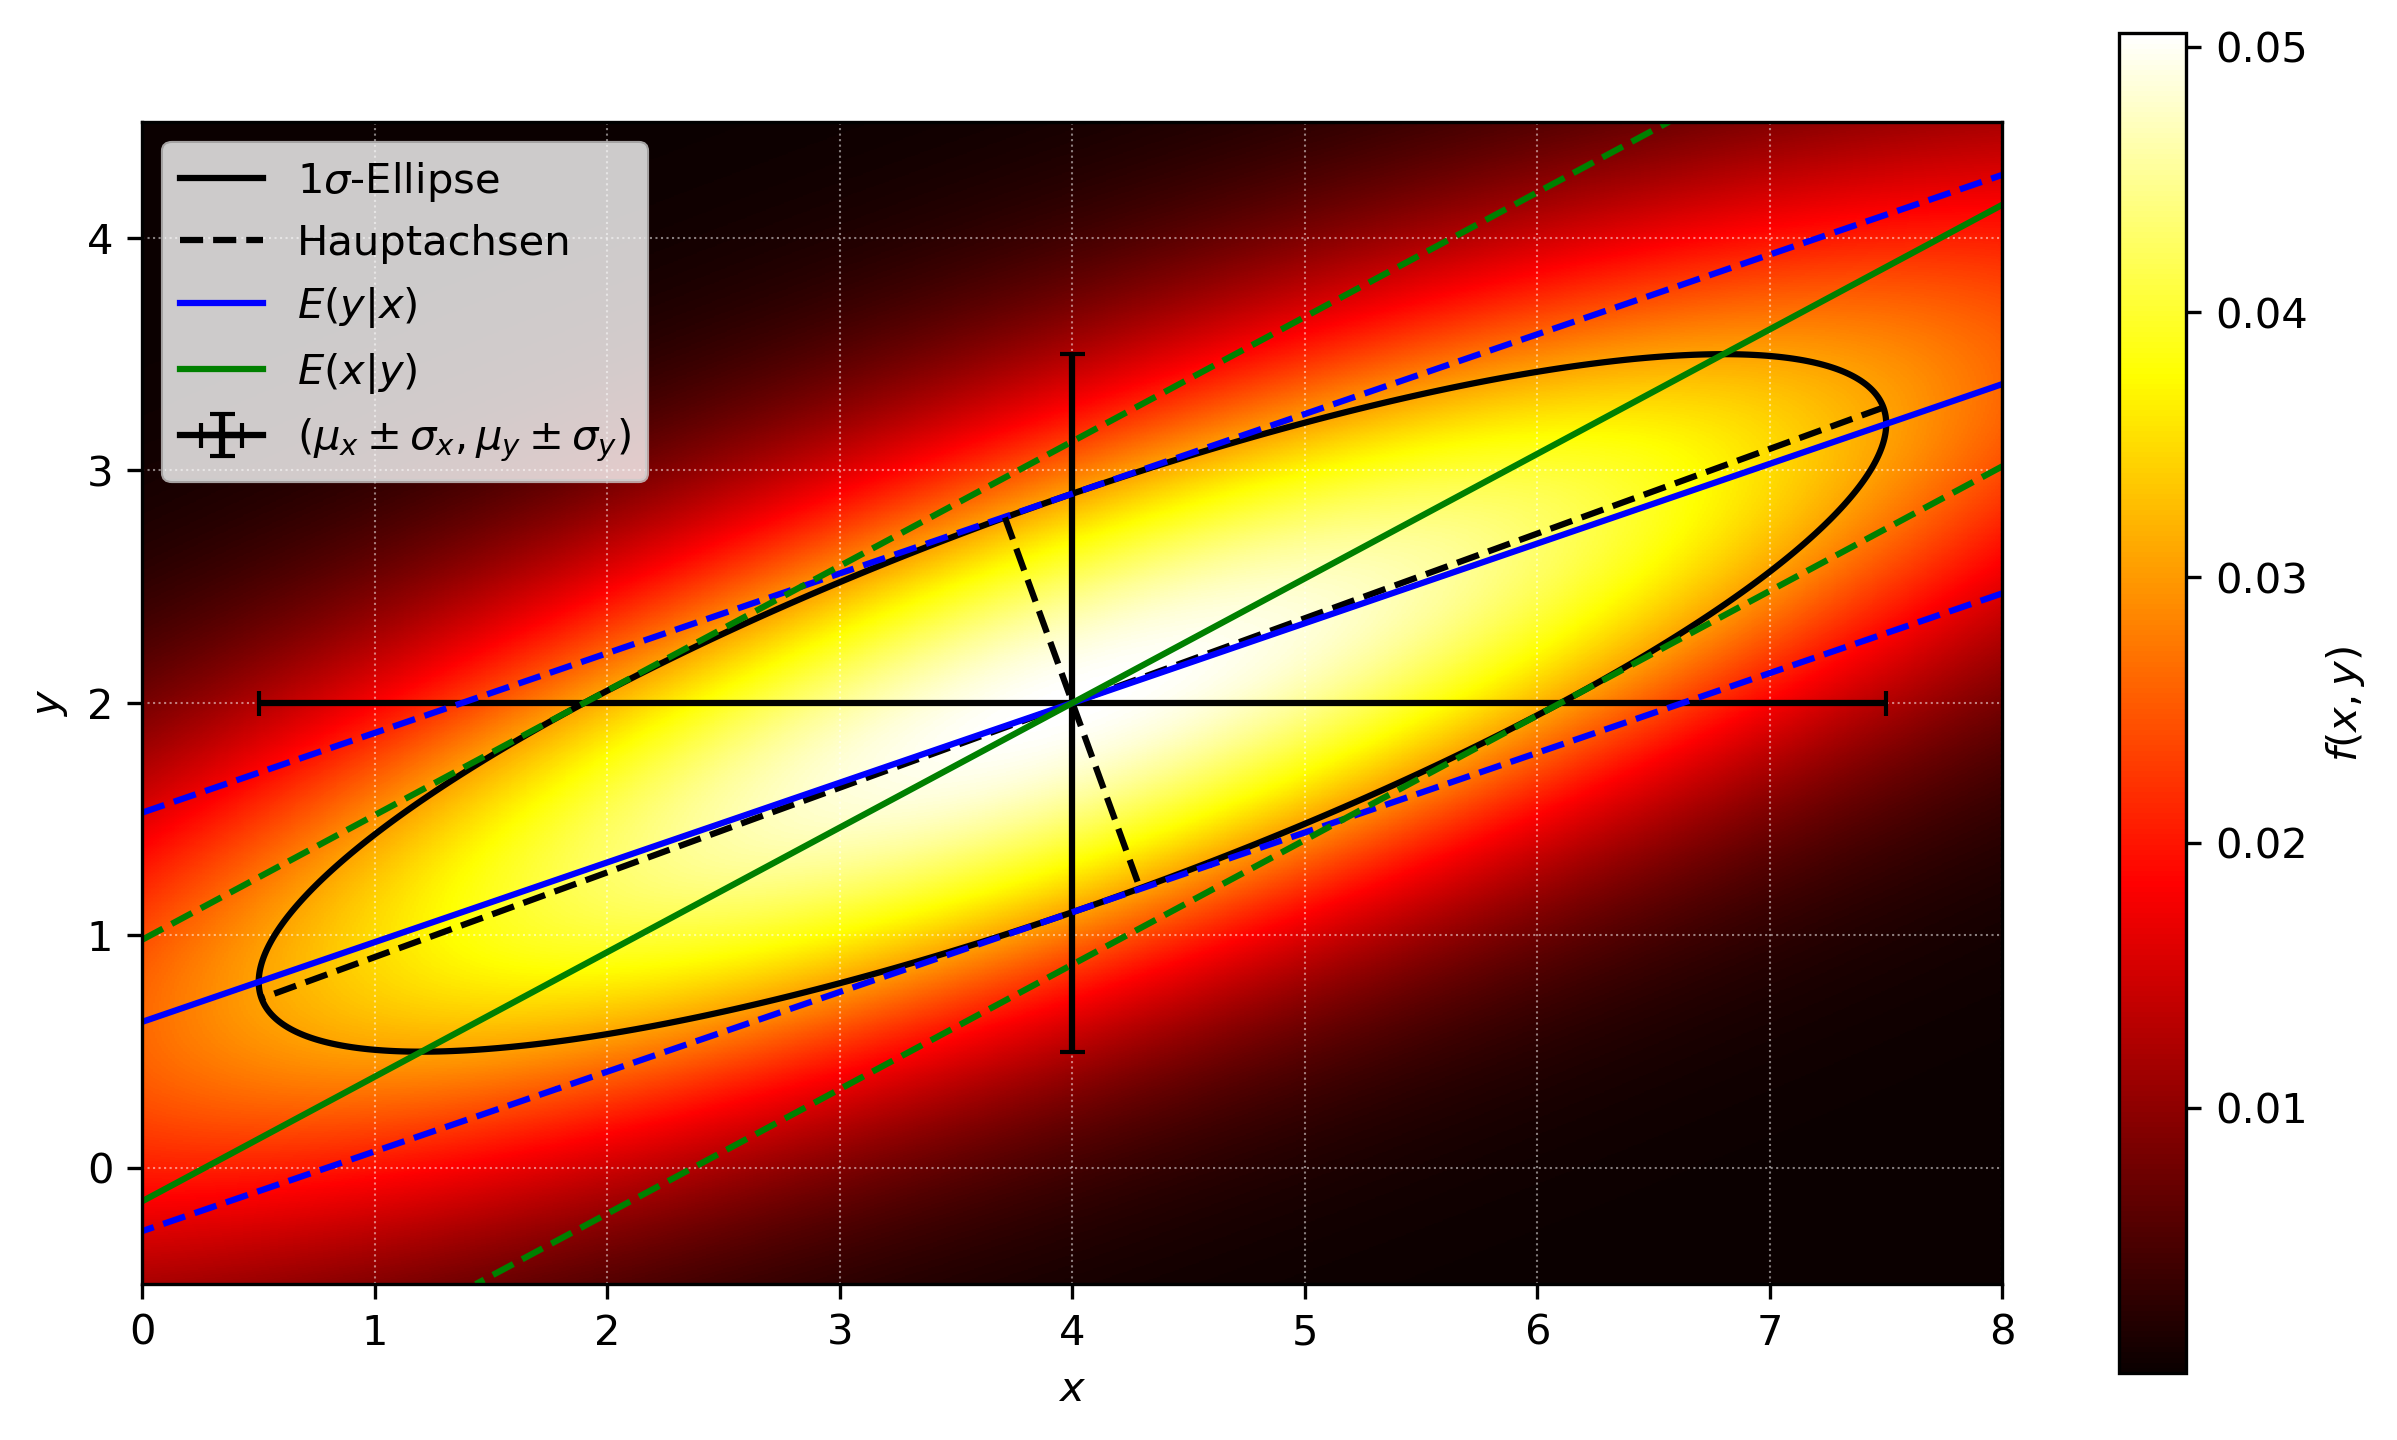
\includegraphics[width=\textwidth]{../A07/A7.png}
    \caption{Graphische Darstellung der Ergebnisse von Aufgabe 7.}
    \label{fig:A7}
\end{figure}
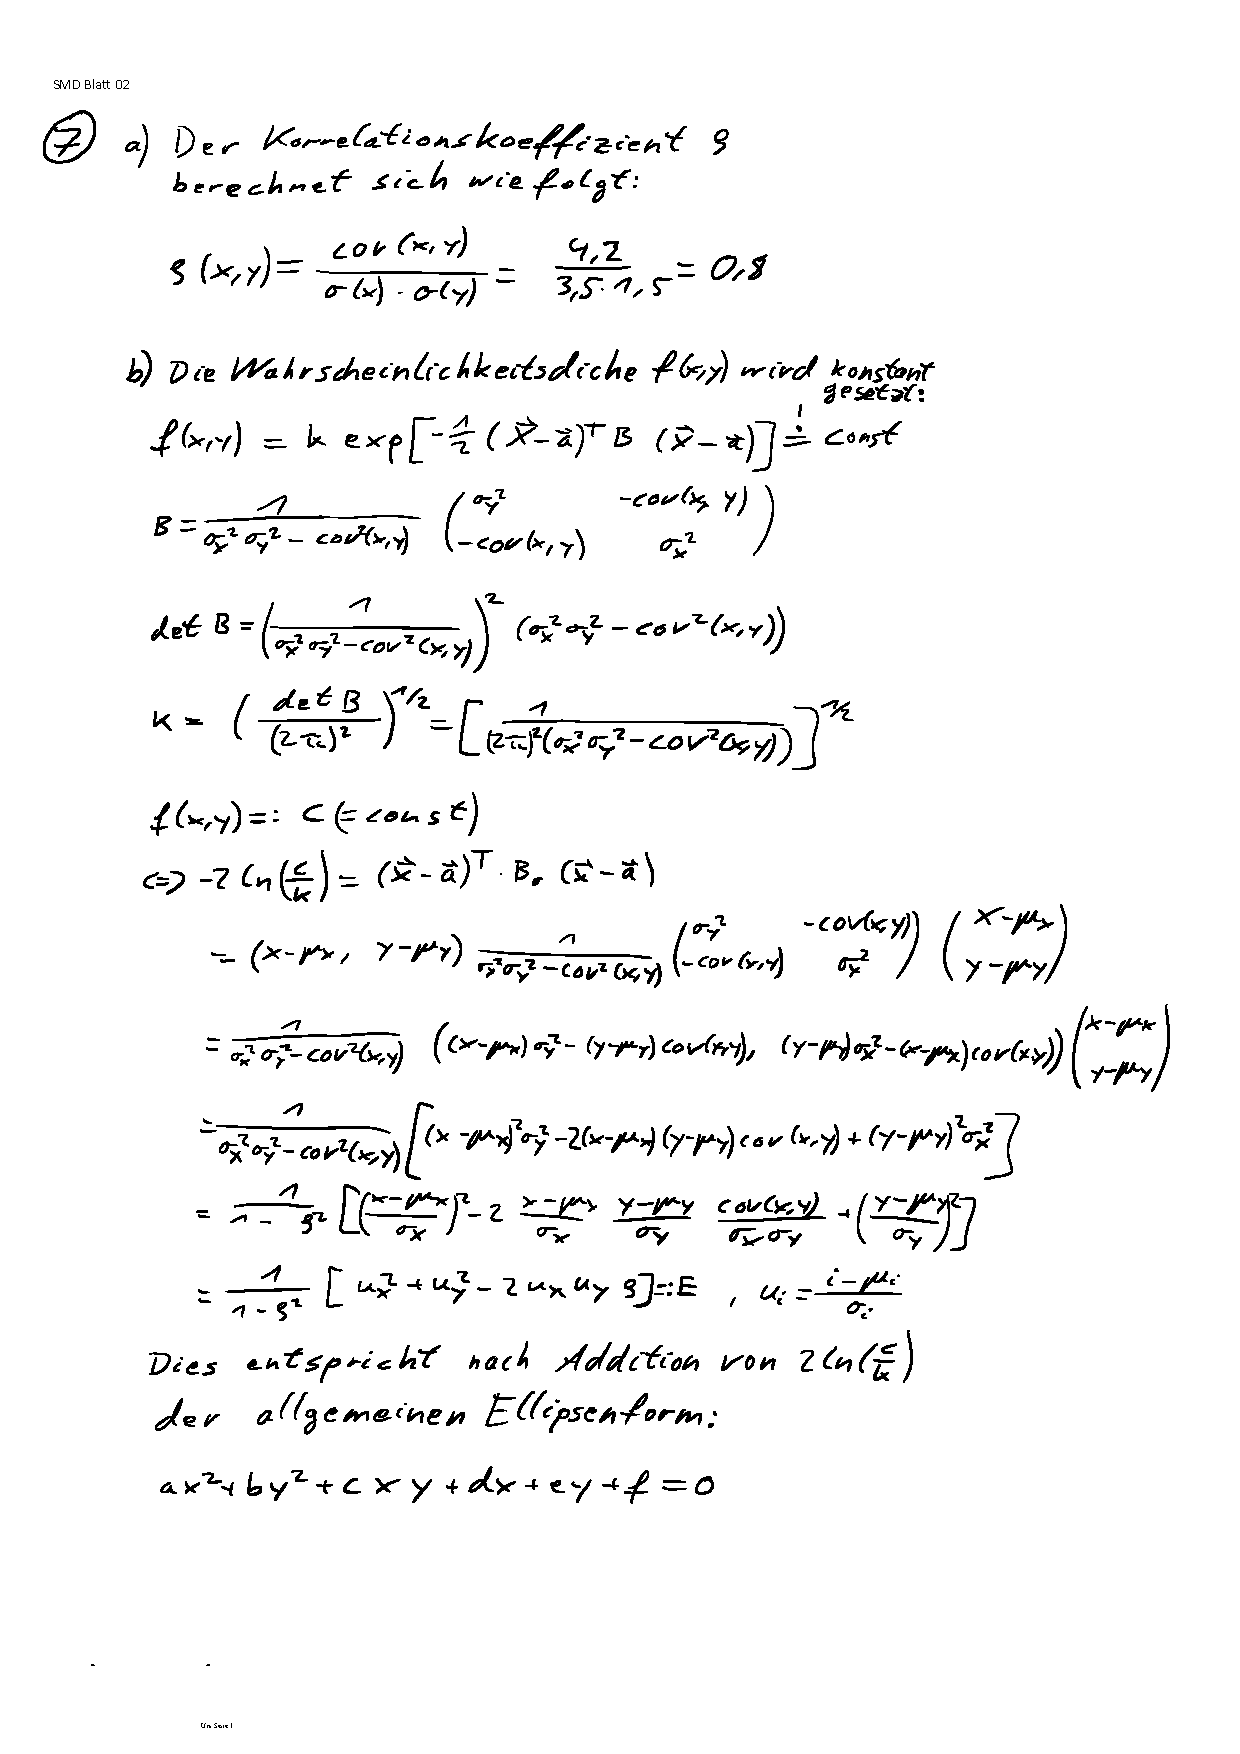
\includepdf[pages=-]{../A07/A7_Text.pdf}
\end{document}
